\section{Модель тонкой мембраны}\label{sec:eq-membrane}
Математическая модель для гибкой мембраны была описана, например в~\cite{rakhmatulin}.

Пусть по гибкой мембране бесконечной протяженности производится прямой удар острым телом, имеющим с ней лишь одну
точку соприкосновения.
Предполагается, что в процессе соударения скорость ударяющего тела $v_0$ остается неизменной, начальная толщина
мембраны $\delta_0$ постоянна, а сама она до удара не деформирована и расположена в одной плоскости.
Для решения поставленной задачи целесообразно ввести цилиндрическую систему координат $(r,y)$ с началом в точке удара,
осью $Or$, расположенной в плоскости мембраны, и осью $Oy$, перпендикулярной к последней и имеющей направление скорости
$v_0$.

Составим уравнения движения элемента гибкой мембраны, вырезанного двумя меридиональными сечениями и двумя сферами,
центры которых лежат на оси $Oy$ и совпадают с вершинами конусов, касающихся указанного элемента.
В силу закона сохранения массы:
\begin{equation}
    \rho_0 \delta_0 r dr d\theta = \rho \delta d\theta \sqrt{\left( 1 + \dfrac{\partial w}{\partial r} \right) ^ 2 + \left( \dfrac{\partial u}{\partial r} \right) ^ 2} dr (r + w)
\end{equation}

Здесь $r$ - координата элемента мембраны до удара (лагранжева координата); $w$, $u$ - соответственно радиальное и
поперечное смещения; $\rho$ - плотность; $\theta$ - полярный угол.

После несложных преобразований получим итоговую систему уравнений:

\begin{equation}
    \rho_0 \left( \dfrac{\partial v_{\tau}}{\partial t} - v_n \dfrac{\partial \gamma}{\partial t} \right) = \dfrac{\partial \sigma_t}{\partial r} + \dfrac{\sigma_t - \sigma_{\theta} \cos{\gamma}}{r}
\end{equation}
\begin{equation}
    \rho_0 \left( \dfrac{\partial v_n}{\partial t} - v_n \dfrac{\partial \gamma}{\partial t} \right) = \sigma_t \dfrac{\partial \gamma}{\partial t} + \dfrac{\sigma_{\theta}}{r} \sin{\gamma}
\end{equation}
\begin{equation}
    \dfrac{\partial v_{\tau}}{\partial r} - v_n \dfrac{\partial \gamma}{\partial r} = \dfrac{\partial e_t}{\partial t} \\
\end{equation}
\begin{equation}
    \dfrac{\partial v_n}{\partial r} + v_{\tau} \dfrac{\partial \gamma}{\partial r} = \left( 1 + e_t \right) \dfrac{\partial \gamma}{\partial t}
\end{equation}
\begin{equation}
    \dfrac{\partial e_{\theta}}{\partial t} = \dfrac{1}{2} \left( v_{\tau} \cos{\gamma} - v_n \sin{\gamma} \right)
\end{equation}


%\section{Моделирование мембраны}\label{sec:model-membrane}
Моделирование мембраны осуществлялось с помощью пакета Comsol Multiphysics.
В результате его работы были получены следующие решения: \picref{pic:comsol-example-1}.

\begin{figure}[H]
    \centering
    \label{pic:comsol-example-1}
    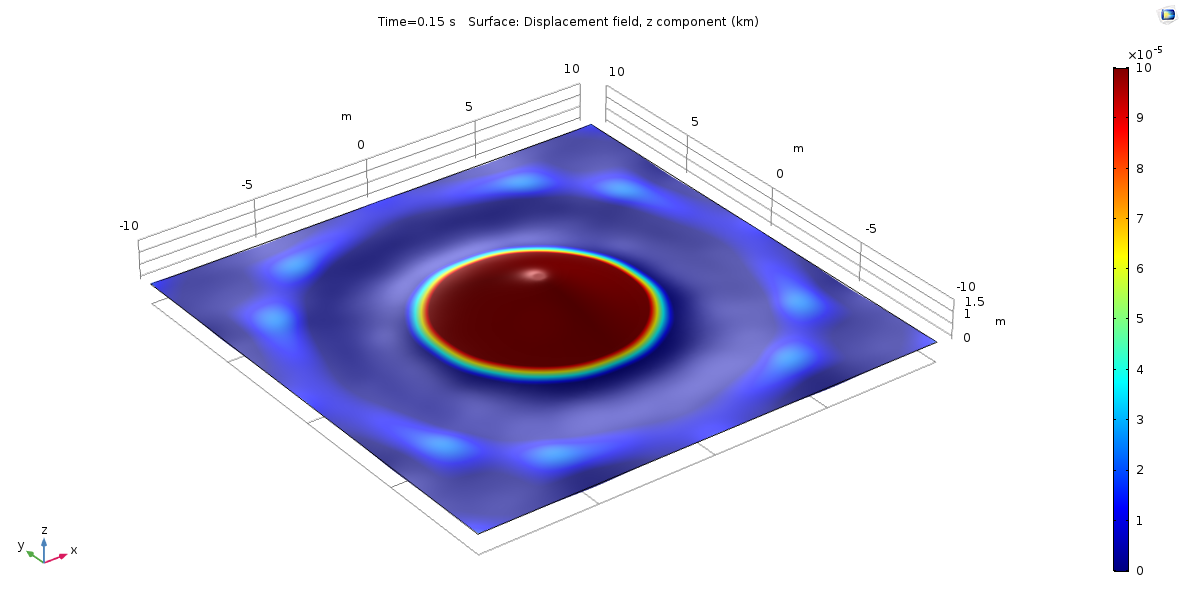
\includegraphics[width=0.8\textwidth]{img/comsol/example_1.png}
    \caption{Деформация изотропной мембраны}
\end{figure}

Данное решение хорошо описывает ожидаемое поведение тканного пакета, но, к сожалению, не даёт простого способа
получить интересующие нас данные по динамике, в частности скорости волнового фронта.

Это приводит нас к необходимости применить методы расчёта для отдельных нитей.

